%%%%%%%%%%%%%%%%%%%%%%%%%%%%%%%%%%%%%%%%%
% Beamer Presentation
% LaTeX Template
% Version 1.0 (10/11/12)
%
% This template has been downloaded from:
% http://www.LaTeXTemplates.com
%
% License:
% CC BY-NC-SA 3.0 (http://creativecommons.org/licenses/by-nc-sa/3.0/)
%
%%%%%%%%%%%%%%%%%%%%%%%%%%%%%%%%%%%%%%%%%

%----------------------------------------------------------------------------------------
%	PACKAGES AND THEMES
%----------------------------------------------------------------------------------------

\documentclass{beamer}

\mode<presentation> {

% The Beamer class comes with a number of default slide themes
% which change the colors and layouts of slides. Below this is a list
% of all the themes, uncomment each in turn to see what they look like.

%\usetheme{default}
%\usetheme{AnnArbor}
%\usetheme{Antibes}
%\usetheme{Bergen}
%\usetheme{Berkeley}
%\usetheme{Berlin}
%\usetheme{Boadilla}
%\usetheme{CambridgeUS}
\usetheme{Copenhagen}
%\usetheme{Darmstadt}
%\usetheme{Dresden}
%\usetheme{Frankfurt}
%\usetheme{Goettingen}
%\usetheme{Hannover}
%\usetheme{Ilmenau}
%\usetheme{JuanLesPins}
%\usetheme{Luebeck}
%\usetheme{Madrid}
%\usetheme{Malmoe}
%\usetheme{Marburg}
%\usetheme{Montpellier}
%\usetheme{PaloAlto}
%\usetheme{Pittsburgh}
%\usetheme{Rochester}
%\usetheme{Singapore}
%\usetheme{Szeged}
%\usetheme{Warsaw}

% As well as themes, the Beamer class has a number of color themes
% for any slide theme. Uncomment each of these in turn to see how it
% changes the colors of your current slide theme.

%\usecolortheme{albatross}
%\usecolortheme{beaver}
%\usecolortheme{beetle}
%\usecolortheme{crane}
%\usecolortheme{dolphin}
%\usecolortheme{dove}
%\usecolortheme{fly}
%\usecolortheme{lily}
%\usecolortheme{orchid}
%\usecolortheme{rose}
%\usecolortheme{seagull}
%\usecolortheme{seahorse}
%\usecolortheme{whale}
%\usecolortheme{wolverine}

%\setbeamertemplate{footline} % To remove the footer line in all slides uncomment this line
%\setbeamertemplate{footline}[page number] % To replace the footer line in all slides with a simple slide count uncomment this line

%\setbeamertemplate{navigation symbols}{} % To remove the navigation symbols from the bottom of all slides uncomment this line
}
\usepackage{graphicx}
\usepackage[mathstyleoff]{breqn}
\usepackage{gensymb}
\usepackage[compat=1.0.0]{tikz-feynman}
\usepackage{tikz}
\usepackage{braket}
\usepackage{graphicx} % Allows including images
\usepackage{booktabs} % Allows the use of \toprule,
\DeclareMathOperator{\Tr}{Tr}
% \midrule and \bottomrule in tables

%----------------------------------------------------------------------------------------
%	TITLE PAGE
%----------------------------------------------------------------------------------------

\title[Entrelazamiento cuántico y el modelo estándar]{Entrelazamiento cuántico y el modelo estándar} % The short title appears at the bottom of every slide, the full title is only on the title page

\author{Óliver Partida Gutiérrez} % Your name
\institute[UNED] % Your institution as it will appear on the bottom of every slide, may be shorthand to save space
{
U.N.E.D \\ % Your institution for the title page
\medskip

}
\date{\today} % Date, can be changed to a custom date

\begin{document}

\begin{frame}
\titlepage % Print the title page as the first slide
\end{frame}

\begin{frame}
\frametitle{Esquema} % Table of contents slide, comment this block out to remove it
\tableofcontents % Throughout your presentation, if you choose to use \section{} and \subsection{} commands, these will automatically be printed on this slide as an overview of your presentation
\end{frame}

%----------------------------------------------------------------------------------------
%	PRESENTATION SLIDES
%----------------------------------------------------------------------------------------

%------------------------------------------------
\section{Introducción} % Sections can be created in order to organize your presentation into discrete blocks, all sections and subsections are automatically printed in the table of contents as an overview of the talk
%------------------------------------------------

%\begin{frame}
%\frametitle{Paragraphs of Text}

%\end{frame}

%------------------------------------------------

%------------------------------------------------
\begin{frame}
\frametitle{Objetivo}
\begin{itemize}
	\item Siguiendo la doctrina \textit{``it from bit''}...
	\item ...analizar hasta que punto un principio de máxima entropía subyace a las interacciones entre partículas.
\end{itemize}
\end{frame}
%------------------------------------------------
\begin{frame}
\frametitle{Principio de máxima entropía}
\begin{itemize}
	\item Propuesto por E.T. Jaynes en 1957.
	\item Dada información testeable sobre una función de probabilidad...
	\item ...seleccionar aquella con mayor incertidumbre consistente con las restricciones.
	\item De esta manera no introducimos supuestos adicionales. 
	\item Maximizar \(S=\sum_{i}p(A_i)\log_2\left(\frac{1}{p(A_i)}\right) \) sujeto a restricciones.
	\item Problema de optimización restringida solucionado mediante multiplicadores de Lagrange.
	
\end{itemize}
\end{frame}

%------------------------------------------------

%------------------------------------------------
\begin{frame}
\frametitle{Entrelazamiento cuántico. Máximo entrelazamiento.}
\begin{itemize}
	\item Fenómeno físico que ocurre cuando un par o grupo de partículas interactuan de tal manera que el estado de cada partícula del par o grupo no puede ser descrito independientemente del estado de las otras.
	\item Aun teniendo toda la información posible del sistema total existe incertidumbre sobre el estado de cada una de las partes que lo componen.
	\item Cada subsistema está en un estado mezcla descrito por una matriz densidad \(\rho = \sum_{j}p_j\ket{j}\bra{j}
	 \).
	\item En sistemas bipartitos, máximo entrelazamiento se corresponde con máxima incertidumbre del estado de cada subsistema.
	\item Entropía de Von Neumann \(S=-\Tr(\rho_A\ln\rho_A)\),
	\item \(\rho_A = \Tr_B(\rho_{AB}) \)
	
	
\end{itemize}
\end{frame}

%------------------------------------------------
%------------------------------------------------
\begin{frame}
\frametitle{Ángulo de Weinberg}
\begin{itemize}
\item Parámetro del modelo estándar \(\theta_W \).
\item Relaciona las partículas mediadoras neutras de la fuerza electrodébil con las del electromagnetismo  y la fuerza nuclear débil.
\[
\quad \left(\begin{array}{@{}c@{}}
B^\mu \\
W_3^\mu
\end{array} \right)
=
\quad
\left(\begin{array}{@{}cc@{}}
\cos\theta_W & -\sin\theta_W \\
\sin\theta_W & \cos\theta_W
\end{array} \right)
\quad
\left(\begin{array}{@{}c@{}}
A^\mu \\
Z^\mu
\end{array} \right),
\]
\item Su valor se obtiene experimentalmente y varía dependiendo de la energía a la que se mida \(Q\).
\item Para \(Q=91.2 GeV/c, \theta_W = 30\degree\).
\end{itemize}
\end{frame}


%------------------------------------------------
\section{Metodología}

%------------------------------------------------

\begin{frame}
\frametitle{\(e^-e^+\rightarrow\mu^+\mu^-\)}
\begin{itemize}
	\item Desintegración electrón positrón para generar un muón y un antimuón.

\end{itemize}
\[
\feynmandiagram [horizontal=a to b] {
	i1 [particle=\(e^{-}\)] -- [fermion,  momentum={\(p\)}] a -- [fermion,rmomentum'={\(p\prime\)}] i2 [particle=\(e^{+}\)],
	a -- [boson, edge label =\(\gamma/Z\), momentum'=\(q\)] b,
	f1 [particle=\(\mu^{+}\)] -- [fermion,rmomentum'={\(k\prime\)}] b -- [fermion,  momentum={\(k\)}] f2 [particle=\(\mu^{-}\)]\text{.}
}; 
\] 
\begin{itemize}
	\item \(\mathcal{M}_{RL}  \sim \alpha_{RL}\ket{RR} + \beta_{RL}\ket{RL} + \gamma_{RL}\ket{LR} + \delta_{RL}\ket{LL}\text{.}\)
\item  Concurrencia \(2|\alpha\delta - \beta\gamma|\text{.}\)

	
\end{itemize}

\end{frame}




%------------------------------------------------
\section{Resultados}
\begin{frame}
\frametitle{Líneas de máximo entrelazamiento}
\begin{figure}[h]
	\centering
	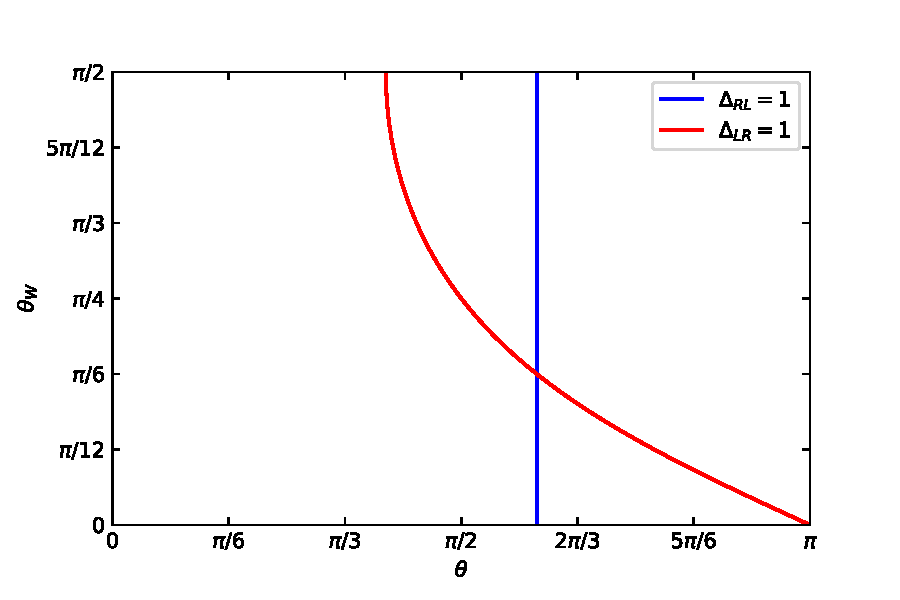
\includegraphics[width=0.85\linewidth]{concurrence.pdf}	
\end{figure}
\end{frame}
\begin{frame}
\frametitle{Conclusiones}
\begin{itemize}
	\item El principio de máxima entropía permite obtener un valor del ángulo de Weinberg, \(\theta_W=\frac{\pi}{6} \), muy cercano al valor real.
	\item Se puede obtener un valor mas exacto teniendo en cuenta términos de mayor orden en la expansión perturbativa.	
	
	
\end{itemize}
\end{frame}

%------------------------------------------------

\begin{frame}
\Huge{\centerline{Muchas gracias por su atención}}
\end{frame}

%----------------------------------------------------------------------------------------

\end{document} 